\chapter{Моделирование излучения FBOT}\label{FBOT}

Последние наблюдения открыли новый класс объектов - быстрые голубые оптические транзиенты (FBOT)\cite{Drout2014, Ho2019cow, Coppejans2020, Ho2020, PerleyCamel, YaoAt2020mrf, MatthewsAT2022tsd, ChrimesAT2023fhn, Perleyvth}. Они характеризуются большой светимостью $L > 10^{43} эрг/с$, смещением цветов в синюю сторону, коротким характерным временным масштабом порядка нескольких дней, низкой выброшенной массой эжекты и её высокими скоростями. Точная природа данных объектов на даный момент неизвестна. Вместе со слабыми гамма-всплесками они возможно принадлежат к переходному классу объектов между нерелятивистскими сверхновыми и обычными гамма-всплесками. Так же возможно их объяснение событиями приливных разрывов.

Рассматриваемый в данной главе объект CSS161010, расположенный в карликовой галактике на расстоянии 150 мегапарсек имеет по оценкам следующие\cite{Coppejans2020} характеристики: скорость эжекты 0.55 c на ранних этапах и около 0.3 c на поздних (порядка одного года), выброшенная масса порядка 0.01-0.1 солнечных масс. Он обладает наибольшей скоростью эжекты из всех известных на текущий момент FBOT объектов, и следовательно наиболее удобен для Particle-in-Cell моделирования в виду малого времени ускорения. \textcolor{red}{Важнейшей особенностью этих объектов является вид их спектральной плотности излучения, имеющей выраженный максимум и степенные участки, говорящие о наличии синхротронного самопоглощения.}
%почему четвертый был отдельно в статье?


В данной главе будет проведено Particle-in-Cell моделирование ускорения частиц в транс-релятивистской ударной волне со скоростями, характерными для FBOT объектов. По имеющимся распределениям будет расчитано синхротронное радио-излучение и с помощью фитирования наблюдательных данных транзиента CSS16 1010 будут подобраны такие параметры как магнитное поле, концентрация вещества и геометрические характеристики в ударной волне. Далее, с использованием широокого распределения частиц, полученного из Монте-Карло моделирования с соответствующими параметрами, будет расчитано рентгеновское излучение от данного объекта.

\section{Излучение объектов с синхротронным самопоглощением}
Процесс синхротронного излучения хорошо известен и описан в классических работах. Но  любому процессу излучения можно так же сопоставить процесс поглощения. Сечение процесса синхротронного самопоглощения описано в работе Гизеллини и Свенсона \cite{Ghisellini1991}. Спектральная плотность мощности излучения единицы объема вещества определеяется формулой
\begin{equation} \label{emission}
I(\nu)=\int_{E_{min}}^{E_{max}} dE \frac {\sqrt {3}{e}^{3}n F(E) B \sin ( \phi)}{{m_e}{c}^{2}}
\frac{\nu}{\nu_c}\int_{\frac {\nu}{\nu_c}}^{\infty }\it K_{5/3}(x)dx,
\end{equation}
где $F\left(E\right)$ - это функция распределения излучающих частиц, $\phi$ - угол межде вектором магнитного поля и лучом зрения, $\displaystyle\nu_{c}$  - критическая частота, определяемая выражением $\displaystyle\nu_{c} = 3 e^{2} B \sin(\phi) E^{2}/4\pi {m_{e}}^{3} c^{5}$, и~$K_{5/3}$ - функция МакДональда.
Коэффициент поглощения для фотонов, распростроняющихся вдоль луча зрения равен
\begin{equation}\label{absorption}
k(\nu)=\int_{E_{min}}^{E_{max}}dE\frac {\sqrt {3}{e}^{3}}{8\pi m_e \nu^2}\frac{n B\sin(\phi)}{E^2}
\frac{d}{dE} E^2 F(E)\frac {\nu}{ \nu_c}\int_{\frac {\nu}{ \nu_c}}^{\infty }K_{5/3}(x) dx.
\end{equation}
Используя эти формулы Шевалье \cite{Chevalier1998} построил модель излучения плоского однородного диска, расположенного перпендикулярно к лучу зрения, с радиусом $R$, толщиной $s$, однородным магнитным полем $B$ и степенной функцией распределения электронов $F(E) = N_0 E^{-p}$. Вместо толщины обычно используется доля излучающего объема $f$, определенная так, что $\pi R^2 s = 4 \pi /3 R^3 f$. При таких предположениях \textcolor{red}{спектральная плотность излучения определяется следующими формулами}
\begin{equation}
I_{\nu}=S(\nu_1)J(\frac{\nu}{\nu_1},p)
{sin(\theta)}^{\frac{p+2}{p+4}},
\end{equation}
где
\begin{equation}
\nu_1 = 2 c_1 {(s c_6 N_0)}^{\frac{2}{p+4}}{B sin(\theta)}^{\frac{p+2}{p+4}}
\end{equation}
\begin{equation}
S(\nu_1)=\frac{c_5}{c_6}{(B sin(\theta))}^{-1/2}{(\frac{\nu_1}{2 c_1})}^{5/2}
\end{equation}
\begin{equation}
J(z,p)=z^{5/2}(1-exp(-z^{(p+4)/2}))
\end{equation}
где $\theta$ - угол между магнитным полем и лучом зрения, $c_1, c_5, c_6$ - константы Пахольчика \cite{Pacholczyk}, зависящие от спектрального индекса электронов.


Измерив спектральную плотность излучения и получив максимум в данный момент времени $F_{max}$, приходящийся на частоту $\nu_{max}$, можно получить размер и магнитное поле в источнике по формулам
\begin{equation}\label{ChevR}
R = {\left( \frac {6 \epsilon_B {c_6}^{p+5}{F_{max}}^{p+6}{
			D}^{2p+12}}{\epsilon_e f \left( p-2 \right) {\pi}^{p+5}{{c_5}}^{p+6}
		{E_1}^{p-2}} \right)} ^{ \frac{1}{p+13} } \frac{2 c_1}{\nu_{max}},
\end{equation}
\begin{equation}\label{ChevB}
B = { \left(\frac {{\epsilon_B}^2 36 {\pi}^{3}{c_5}}{{
			\epsilon_e}^{2}{f}^{2} \left( p-2 \right) ^{2}{{c_6}}^{3}{{E_1}}^{2 p-4}F_{max}{D}^{2}} \right)}
^{\frac{2}{2p+13}}\frac{\nu_{max}}{2 c_1},
\end{equation}
где $D$ - расстояние до источника, $\epsilon_B, \epsilon_e$ - доли энергии в источнике, содержащиеся в магнитном поле и в электронах, $E1$ - энергия, с которой начинается степенное распределение электронов. Таким образом в работах  были оценены параметры источников AT2018cow \cite{Ho2019cow}, CSS161010 \cite{Coppejans2020}, ZTF2018abvkwla \cite{Ho2020} и AT2020xnd \cite{Ho2021, Bright2021}. Так же, измеряя размер источника $R$ в разные моменты времени можно оценить скорость распространения ударной волны.
\section{Particle-in-Cell моделирование }
Для более точного расчета синхротронного излучения оптических транзиентов необходимо знание функции распределения электронов. В перечисленных выше работах используется модель степенного распределения с произвольным параметром - долей энергии в электронах $\epsilon_e$, но как показано в работе \cite{Margalit2021}, тепловые электроны так же могут вносить значительный вклад в излучение. Мы для определения функции распределения электронов в субрелятивистской ударной волне использовали Particle-in-Cell расчеты, выполненные с помощью кода Smilei \cite{Smilei18}, разработанным Деруле и другими. Этот код основан на явной конечно-разностной схеме, с релятивистскими уравнениями движения и с алгоритмом сохранения заряда, предложенным Езиркеповым \cite{Esirkepov}.

Для инициализации ударной волны мы используем распространенный подход - в двумерной симуляции на левой границе по оси $x$ установлена отражающая стенка, с которой сталкивается однородный поток плазмы. На правой границе использованы граничные условия сохраняющие поток. Вдоль перпендикулярного направления $y$ установлены периодические граничные условия. Все вектора, кроме координат частиц - поля и скорости, являются трехмерными, так называемая 2d3v схема. Число ячеек в продольном направлении 
$\displaystyle Nx = 204,800$, в поперечном $\displaystyle Ny = 400$. Размер ячейки $dx = dy = 0.2c/{\omega_e}$ , где $\displaystyle\omega_e$ - плазменная электронная частота $\displaystyle\omega_e = \sqrt{4 \pi n e^2/ m_e}$, $\displaystyle e$ - абсолютная величина заряда электрона, $\displaystyle n$ - концентрация (в коде SMILEI может быть выбрана произвольно, другие величины легко масштабируются), $\displaystyle m_e$ - масса электрона, увеличена для экономии численных ресурсов так, что отношение масс протона и электрона $m_p/m_e = 100$. Начальное магнитное поле $\displaystyle\vec{B}$ лежит в плоскости симуляции под углом $\displaystyle\theta$ к скорости потока. Электрическое поле инициализируется так, чтобы компенсировать силу Лоренца в лабораторной системе $\displaystyle\vec{E} = -\vec{v} \times
\vec{B}/c$. Скорость потока плазмы $\displaystyle v$  is $0.3 c$ 
что соответствует лоренц-фактору $\displaystyle\gamma = 1.05$. Такая скорость соответствует оценкам для выбранного нами транзиента CSS161010 из статьи \cite{Coppejans2020}. Замагниченность потока $\displaystyle\sigma = B^2/4 \pi n \gamma m_p c^2 = 10^{-4}$. С такими параметрами размер области симуляции вдоль оси $\displaystyle x$ соответствует $\displaystyle 500$
гирорадиусам протонов в потоке плазмы $\displaystyle r_g = m_p v c \gamma/e B$, а вдоль оси $\displaystyle y$ одному гирорадиусу. Максимальное время симуляции составляет $\displaystyle 7\times 10^4~\omega_{e}^{-1}$ или около
$\displaystyle 100$ обратных протонных гирочастот. Для концентраций порядка $\displaystyle n\approx
1$~cm$^{-3}$, это время соответствует временам порядка одной секунды, что намного меньше характерного времени активного излучения быстрых оптических транзиентов, а значит такое квазистационарное моделирование применимо к рассматриваемому объекту в каждый отдельный момент времени.

Эффективность ускорения частиц зависит от угла наклона магнитного поля $\displaystyle\theta$,
особенно в случае релятивистских ударных волн \cite{SironiSpitkovsky2009pair, GuoSironi2014_1, Crumley2019, Romansky2018}. Чтобы быть вовлеченной в процесс ускорения Ферми первого рода, частице необходимо удалиться от фронта, и если
она движется вдоль силовых линий магнитного поля, максимальная возможная скорость вдоль оси $\displaystyle x$ равна $\displaystyle c\cos(\theta')$, и для ухода от ударной волны она должна быть больше скорости самой ударной волны $\displaystyle v_{sh}'$ (все величины измерены в системе набегающего потока). Поэтому для квазипоперечных ударных волн, у которых $c \cos(\theta')$ меньше скорости ударной волны $\displaystyle v_{sh}'$ ускорение невозможно. При углах наклона меньших критического, ударная волна способна эффективно ускорять частицы и формировать степенной хвост их функции распределения. Проводились расчеты со скоростями натекающего потока 0.5 c, 0.75 c и углами наклона магнитного поля от 10 до 90 градусов. Полученные функции распределения протонов и электронов представлены на рисунках \ref{distributionsE} и \ref{distributionsP}.
\begin{figure}[h]
	\begin{minipage}{0.49\textwidth}
	\centering
	\includegraphics[width=0.95\textwidth]{./img_part1/electrons_momentum.png} 
	\caption{Функции распределения электронов за фронтом ударных волн с различными углами наклона магнитного поля  $\theta$ и скоростями $v$}
	\label{distributionsE}
    \end{minipage} \hfill
    \begin{minipage}{0.49\textwidth}
	\centering
	\includegraphics[width=0.95\textwidth]{./img_part1/protons_momentum.png} 
	\caption{Функции распределения протонов за фронтом ударных волн с различными углами наклона магнитного поля $\theta$ и скоростями $v$}
	\label{distributionsP}
    \end{minipage}
\end{figure}
 
%Для дальнейшего моделирования излучения использовалась функция распределения, полученная для угла $\theta = 30^\circ$ градусов (квазипараллельная ударная волна).
 
%Из результатов моделирования можно извлечь параметры полученного распределения электронов. За фронтом ударной волны функция распределения электронов имеет сложный вид, но можно выделить две основных компоненты - тепловой пик и степенной хвост на высоких энергиях.
%На низких энергиях ($\displaystyle E < 5 m_e c^2$) мы аппроксимируем фунцию распределения с помощью распределения Максвелла-Юттнера, итеративным процессом минимизируя функционал $\displaystyle f(T) = \int_{m_e c^{2}}^{5 m_e c^{2}} (F(E) - F_{mj}(E,T))^{2}dE$, где $\displaystyle F(E)$ функция распределения полученная из моделирования, $\displaystyle F_{mj}(E,T)$ - распределение Максвелла-Юттнера. Таким образом определяется температура, соответствующая тепловому пику. Для высоких энергий ($\displaystyle 20~m_e c^{2} < E < 50~m_e c^{2}$) мы используем линейную регрессию в дважды логарифмических координатах для определения спектрального индекса $p$. Функция распределения электронов за фронтом ударной волны (от 2000 до 5000 ячеек за фронтом) в момент времени $\displaystyle t$ = 70,000~$\omega_{e}^{-1}$ при начальных параметрах $\displaystyle\sigma = 0.0002$, $\theta = 30^\circ$ и ее аппроксимации с \textcolor{red}{температурой $\displaystyle T_e = 5\times 10^{10}$~K} и спектральным индексом $\displaystyle p = 3.6$ изображены на рисунке ~\ref{electrons}.
%Так же с помощью Particle-in-Cell моделирования можно определить параметры $\epsilon_B, \epsilon_e$, определяющие связь между концентрацией и магнитным полем, которые необходимы для дальнейшего расчета излучения.
%\begin{figure}
%		\centering
%		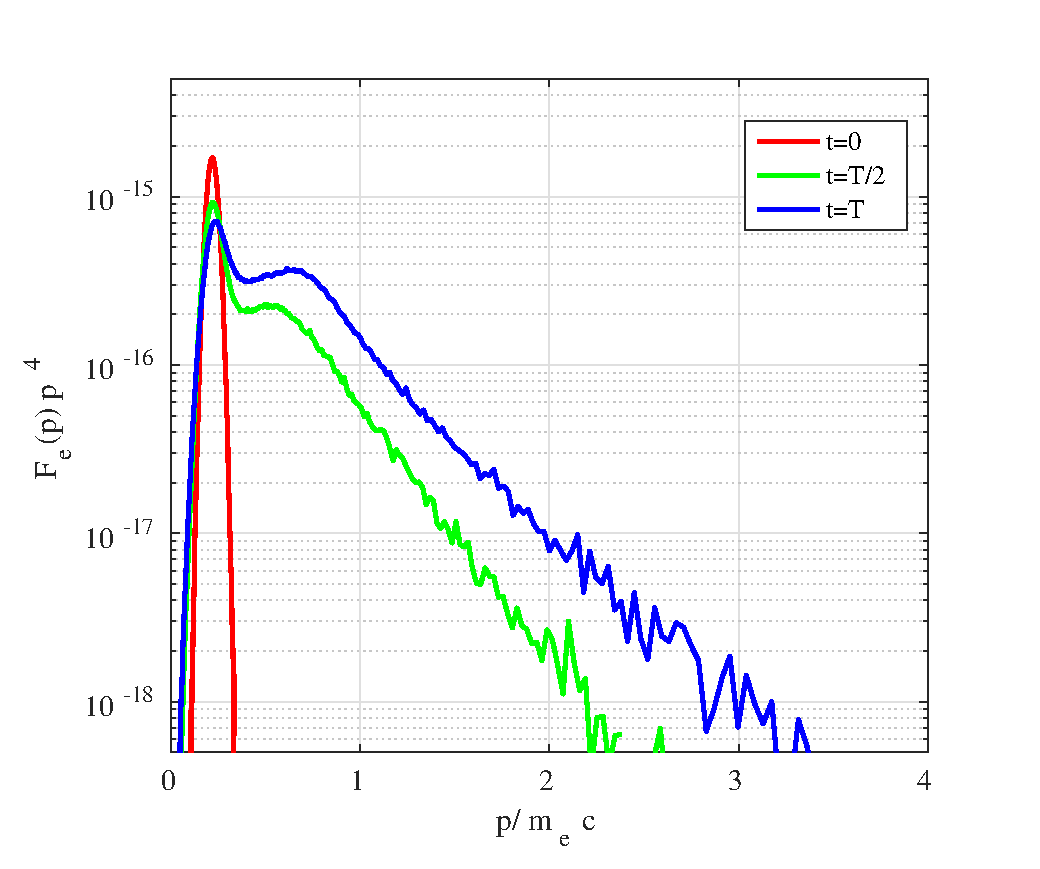
\includegraphics[width=10.5 cm]{electrons.eps} 
%		\caption{Функция распределения электронов за фронтом ударной волны при начальных параметрах $v = 0.3~c,$ $\sigma = 2\times10^{-4}$ и $\theta = 30^{\circ}$.}
%		\label{electrons}
%\end{figure}

%\section{Расчёт излучения}

\section{Фитирование парметров радиоисточника}

Зная точную функцию распределения и предположив геометрию источника в виде плоского диска, можно рассчитать наблюдаемые потоки с помощью известных формул для синхротронного излучения и самопоглощения, описанных например в работе \cite{Ghisellini}. 
Проинтегрировав излучательную способность по объему с учетом самопоглощения (формулы \ref{emission} и \ref{absorption}) и зная расстояние $\displaystyle D$ до источника, можно определить спектральную плотность потока излучения.

Были проведены расчеты синхротронного излучения и подбор параметров для оптического транзиента CSS161010 для моментов времени $\displaystyle t = 69, 99 и 357$ дней после взрыва, для четырех функций полученных из PIC моделирования - для скоростей потока 0.5 c и 0.75 c и для углов наклона 30 и 80 градусов. Полученные значения функционала и параметров для разных моделей для момента времени 99 дней после взрыва показаны в талблице \ref{parameters}.

\textcolor{red}{написать про толщину 0.1 а не 0.5}

\renewcommand{\arraystretch}{1.375}
\begin{table}[h!]
	\label{parameters}
	\caption{Полученные значения параметров радиоисточника для различных моделей}
	\begin{center}
		\begin{tabular}{|c | c| c| c| c| c|}
			\hline
			model &$r$ & $B$, G& $n$,~$\rm cm^{-3}$&  $E_e,~\rm erg$& $E_p,~\rm erg$\\
			\hline
			A80 & 550 & 0.5 & 2$\times 10^6$  & 3.4$\times 10^{51}$ & 3$\times 10^{53}$\\
			\hline
			A30 & 140 & 0.1& 5$\times 10^5$&  8$\times 10^{51}$ & 7$\times 10^{53}$\\
			\hline
			B80 & 170 & 0.3& 540&  3$\times 10^{49}$& 3.7$\times 10^{51}$\\
			\hline
			B30 & 57 & 0.34& 17&  2.2$\times 10^{48}$& 1.4$\times 10^{50}$\\
			\hline
		\end{tabular}
	\end{center}
\end{table}

Полученные значения магнитного поля и концентрации в лучше всего подходящей модели B30 близки к полученным авторами оригинальной работы \cite{Coppejans2020} с помощью уравнений~(\ref{ChevR})
и (\ref{ChevB}), в предположении равенства распределения энергий $\epsilon_e = \epsilon_B = 1/3$, в то время как скорость и соответственно размер источника оказываются значитеьно большими.
Для этой же модели B30 проведено фитирование параметров в другие моменты времени, получены следующие значения. На 69-ый день магнитно поле равно $0.4~\rm G$, концентрацияя $24~\rm cm^{-3}$ , а размер источника $R =1.3\times10^{17}~\rm{cm}$. На 357-ой день магнитное поле равно $0.04~\rm G$, концентрация $0.25~\rm cm^{-3}$, а размер источника $R= 6.9\times10^{17}~\rm{cm}$. Полученные значения магнитного поля и концентрации значительно отличаются от простых ожидаемых зависимостей от расстояния $B \propto r^{-1}$ and $n  \propto r^{-2}$, а так же попытка одновременного фитирования всех трех моментов времени со степенными зависимостями размера от времени и магнитного поля и концентрации от расстояния не удалась, что может говорит о сильной неоднородности и немонотонности плотности вокруг источника.

Расчеты были проведены для трех конфигураций источника - степенной функцией распределения и параметрами из статьи \cite{Coppejans2020}, с функцией распределения, полученной из PIC моделирования, и с функцией с экстраполированным степенным хвостом до энергий $\displaystyle 500~m_{e} c^{2}$. В последних двух случаях размер источника и магнитное поле подбирались минимизацией функционала $\displaystyle g(B,R) = \sum (F(\nu_{i}, B, R) - F_{obs}(\nu_{i}))^{2}$, где $\nu_i$ 
наблюдаемые частоты, $\displaystyle F_{obs}(\nu_{i})$ наблюдаемые потоки
$\displaystyle F(\nu_{i}, B, R)$---рассчитанные потоки.
Мы использовали шесть измерений из ~\cite{Coppejans2020}: четыре сделанные VLA на 357-ой день
на частотах 1.5, 3.0, 6.05 и 10~GHz и два сделанные GMRT на 350-ый день на частотах 0.33 и 0.61 GHz. Результаты расчетов излучения показаны на рисунке \ref{radiation}.
Как можно видеть из рисунка, модель с функцией распределения полученной непосредственно из PIC расчетов не может объяснить наблюдаемое излучение. Но так как время расчетов намного порядков меньше времени наблюдения источника, мы считаем возможным экстраполировать степенной хвост функции распределения до более высоких энергий. Такая экстраполированная функция распределения, как и чисто степенная, хорошо объясняют наблюдения. Но полученные физические параметры источника оказываются существенно различными. Магнитное поле $\displaystyle B = 0.069$~G, и радиус источника $\displaystyle R = 3.0 \times
10^{17}$~cm близки к значениям из статьи \cite{Coppejans2020}, в то время как полученное значение концентрации $\displaystyle n = 210$~cm$^{-3}$ оказывается значительно больше.
\begin{figure}
	\centering
	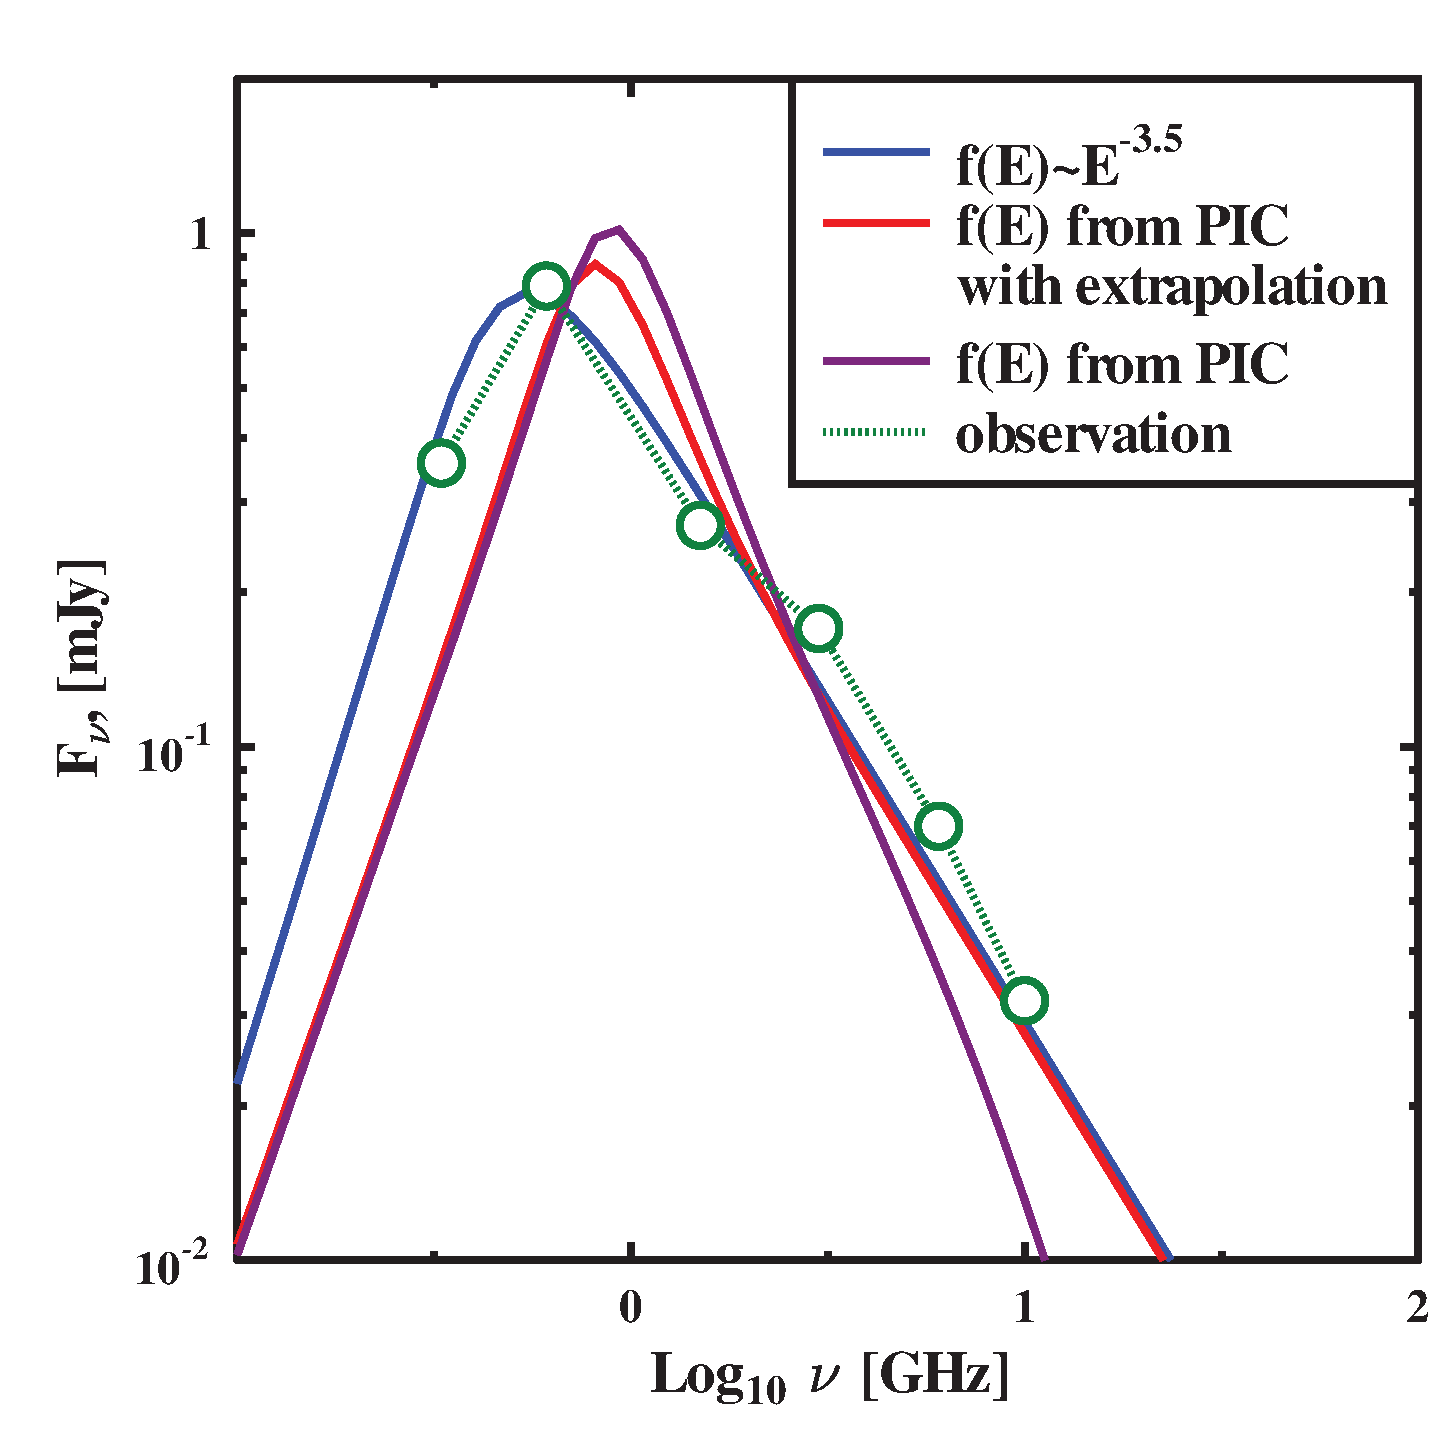
\includegraphics[width=10.5 cm]{radiation.eps} 
	\caption{Наблюдаемые 
		(зеленые круги) и расчетные спектральные плотности излучения CSS161010  на 357-ой день для разных моделей распределения электронов.} 
	\label{radiation} 
\end{figure} 

\section{Расчет рентгеновского излучения}
На 99-ый день с момента детектирования имеются одновременные наблюдения в радио и в рентгеновском диапазоне. Объект обладает большой рентгеновской светимостью (поток $F_{X} = (1.33 \pm 0.76)\times10^{-15} ~\rm erg~s^{-1}~cm^{-2}$ и соответствующая изотропная светимость $L_{X}=(3.4\pm1.9)\times10^{39}~\rm erg~s^{-1}$ iв диапазоне $0.3-10~\rm keV$ \cite{Coppejans2020}). Последние исследования FBOT предполагают наличие центрального источника для объяснения рентгеновского излучения --- предполагается, что на ранних стадиях оно производится милисекундным магнетаром \citep{GottliebFBOTjet}, а на поздних стадиях аккреционным диском \citep{MiglioriFBOtlatestages}. Мы далее предлагаем модель объясняющую рентгеновское излучение FBOT (конкретно CSS161010) без центрального источника, по крайней мере на поздних стадиях.

Если продлить степенное распределение электронов (с показателем спектра $\approx3.5$), полученное из PIC моделирования, до высоких энергий, то полученный уровень рентгеновского излучения за счет синхротронного механизма окажется на несколько порядков ниже наблюдаемого. Но как следует из Монте-Карло расчетов, на высоких энергиях спектр ускоренных частиц становится более жестким. Монте-Крло моделирование не рассматривает электроны, но в диффузионном приближении функция распределения на высоких энергиях определяется только коэффициентом диффузии, который мы берем зависящим только от гирорадиуса частцы, и являющегося одинаковым для пртонов и электронов с одной энергией. Поэтому функции распределения протонов и электронов будут подобны до тех пор, пока синхротронные потери не начнут играть роль. Ограничения за счет синхротронных потерь можно вычислить оценив максимальную достижимую энергию, сравнив темп набора энергии и темп синхротронных потерь. 

\begin{equation} \label{accTime}
	t_{acc}=\int_{p_0}^p \frac{3}{v_1-v_2}\left(\frac{D_1}{v_1}+\frac{D_2}{v_2}\right)\frac{dp}{p}
\end{equation}

где $D_1, D_2$ коэффициенты диффузии, $v_1, v_2$ --- скорости потока перед и за фронтом ударной волны соответственно \citep{Drury83}. Для релятивистской частицы , ускоряющейся на сильной ударной волне с бомовским коэффициентом диффузии  $D = cE/3eB$, можно получить скорость набора энергии $dE_{acc}/dt = 3 v^2 e B/8c$. Приравняв это к скорости синхротронных потерь получим максимальную достижимую энергию электронов $E_{max}= (v/c) \cdot m^2 c^4/\sqrt{e^3 B}$. В нашей модели магнитное поле $B\approx0.3~\rm{G}$ и соответствующее значение максимальной энергии $E_{max}$ равно $\approx10^8~m_e c^2$. Таким образом, скорректируем функцию распределения электронов, домножив функцию распределения протонов на $\exp(-E/E_{max})$. Абсолютную величину высокоэнергичной части функции распределения электронов получим экстраполируя низкоэнегричную часть, полученную из PIC моделирования, до энергий больших энергии тепловых протонов.

Была проведена серия Монте-Карло расчетов, со скоростью ударной волны и концентрациями, соответствующими модели B30 и различными значениями начального магнитного поля, так, чтобы в результате усиления магнитного поля, получилось значение так же соответствующее модели B30. Это происходит при величине начального поля $3\times10^{-5}~G$. Функция распределения из данного расчета была использована для получения композитных функция распределения протонов и электронов, изображенных на рисунке \ref{distributions}. Отличие в уровне инжекции протонов и электронов оказывается $\sim 2\times10^3$ что соотвтетствует результатам, полученным в работе \cite{ParkElectronIonShock}.



\begin{figure}
	\centering
	\includegraphics[width=0.8\textwidth]{./img_part1/distributions2_momentum.png} 
	\caption{Функции распределения протонов и электронов, полученные объединением результатов PIC и МОнте-Карло моделирования со скоростью ударной волны 0.75 c. Пунктирная линия означает функцию распределения электронов без учета синхротронных потерь, а широкая голубая линия - область сшивки двух распределений.}
	\label{distributions}
\end{figure}

Для расчета высокоэнергичного излучения необходимо учитывать пространственную неоднородность функции распределения за счет потерь при движении от фронта ударной волны. Пренебрежем диффузионным переносом и будет расчитывать аналитически конвекционный перенос с синхротронными потерями. Тогда на расстоянии $l$ от фронта ударной волны функция распределения будет выражаться через функцию распределения на фронте $f(E)$ как

\begin{equation}
	f_l(E)=f\left(\frac{E}{1-4e^4 B^2 E~l/9m^4 c^7 u_d}\right)\cdot\frac{1}{\left(1-4e^4 B^2 E~l/9m^4 c^7 u_d\right)^2}
\end{equation}

где $u_d$ - скорость потока в даунстриме, равная 0.2 c в нашей модели. Спектр синхротронного излучения источника в широком диапазоне энергий приведен на рисунке \ref{long_radiation}. Низкочастотный пик связан с синхротронным самопоглощение в радиодиапазоне, второй пик связан с укручением спектра электронов на высоких энергиях, а спад - с завалом функции распределения за счет синхротронных потерь. Полученное значение потока в диапазоне $0.3-10~\rm keV$ равно $8.9\times10^{-16}~\rm erg~cm^{-2} s^{-1}$. Это значение согласуется с наблюдаемым рентгеновским потоком от CSS161010 на 99-ый день после взрыва.

\begin{figure}
	\centering
	\includegraphics[width=0.8\textwidth]{./img_part1/long_radiation.png} 
	\caption{Модельный спектр излучения синхротронного излучения с учетом композитной функции распределения электронов. Интегральны рентгеновский поток в диапазоне $0.3-10~\rm keV$ равен $8.9\times10^{-16}~\rm erg~cm^{-2} s^{-1}$ что соответствует наблюдаемому Чандрой значению $F_{X} = (1.33 \pm 0.76)\times10^{-15} ~\rm erg~s^{-1}~cm^{-2}$.}
	\label{long_radiation}
\end{figure}


\FloatBarrier
\section{Заключение}
 

Получены следующие результаты:
\begin{enumerate}
\item 
\item 
\end{enumerate}


\clearpage